\documentclass[theme=teal]{khmermath}
\usepackage{needspace}
\geometry{left=0.85cm, right=0.85cm, top=0.70cm, bottom=1.35cm, footskip=0.65cm}
\usepackage{colortbl}
\usepackage{tikz}
\usetikzlibrary{calc,shapes,arrows,intersections,through,backgrounds,shadows,decorations.pathmorphing,angles,quotes}

% Define arc accent
\newcommand{\wideparen}[1]{\overset{\boldsymbol{\frown}}{#1}}

% -------------------------------------------------------------------------
% Korean Math Textbook Style Color Palette & Macros
% -------------------------------------------------------------------------
\definecolor{koreaTeal}{RGB}{0, 150, 155}       % Primary Header Teal/Cyan
\definecolor{koreaDarkTeal}{RGB}{0, 105, 110}   % Dark Teal Accent
\definecolor{koreaBeige}{RGB}{247, 244, 237}     % Concept Sidebar Beige
\definecolor{koreaBeigeBorder}{RGB}{225, 218, 205}
\definecolor{koreaOrange}{RGB}{235, 115, 30}     % Problem Number Orange
\definecolor{koreaBlue}{RGB}{35, 110, 190}      % Standard Blue
\definecolor{koreaPurple}{RGB}{125, 50, 160}    % Purple Accent
\definecolor{koreaNumber}{RGB}{115, 125, 135}   % Problem Number Gray
\definecolor{koreaYellow}{RGB}{255, 246, 175}   % Yellow Highlight Tint

\definecolor{brandNavy}{RGB}{0, 105, 110}
\definecolor{brandBlue}{RGB}{0, 150, 155}
\definecolor{brandLightBlue}{RGB}{247, 244, 237}
\definecolor{brandCrimson}{RGB}{195, 35, 60}
\definecolor{brandCoral}{RGB}{235, 80, 75}
\definecolor{brandGold}{RGB}{215, 130, 10}
\definecolor{brandGoldBg}{RGB}{255, 252, 242}
\definecolor{brandTeal}{RGB}{0, 150, 155}
\definecolor{brandTealBg}{RGB}{244, 252, 250}
\definecolor{subtleGray}{RGB}{246, 251, 249}
\definecolor{cardBorder}{RGB}{220, 212, 198}
\definecolor{treeGreen}{RGB}{34, 139, 34}
\definecolor{treeBrown}{RGB}{139, 69, 19}

% Custom Header & Footer setup (Korean Textbook Style)
\usepackage{fancyhdr}
\pagestyle{fancy}
\fancyhf{}
\renewcommand{\headrulewidth}{0pt}
\renewcommand{\footrule}{\color{koreaTeal!60}\hrule height 0.6pt\vspace{2.5pt}}

\fancyfoot[L]{%
  \fontsize{8.5}{8.5}\selectfont\kml \color{koreaNumber}\textbf{\thepage}\ \vline\ \color{koreaDarkTeal}\textbf{១៧. ពហុកោណ}%
}
\fancyfoot[C]{%
  \fontsize{8.5}{8.5}\selectfont\kby \color{koreaDarkTeal}\textbf{\ding{72}\ បង្រៀនដោយ ៖ \textcolor{koreaDarkTeal}{ក្រូត រស្មី}\ \ding{72}}%
}
\fancyfoot[R]{%
  \fontsize{8.5}{8.5}\selectfont\kby \color{koreaDarkTeal}\textbf{ Telegram: \textcolor{brandCrimson}{070897540}}\ \vline\ \color{koreaNumber}\textbf{\thepage}%
}

% Korean Header Banner
\newcommand{\koreanheader}[2]{%
  \noindent%
  \begin{tikzpicture}[x=1cm, y=1cm]
    \fill[koreaTeal, rounded corners=12pt] (0, 0.1) -- (0, 0.95) -- (3.8, 0.95) [rounded corners=0pt] -- (4.4, 0.1) -- cycle;
    \node[white, font=\fontsize{11}{11}\selectfont\kml\bfseries] at (1.9, 0.52) {#1};
    \node[anchor=west, font=\fontsize{17}{17}\selectfont\kml\bfseries, color=koreaDarkTeal] at (4.6, 0.42) {#2};
    \node[anchor=east, font=\fontsize{8.5}{8.5}\selectfont\kby, color=gray!80] at (19.2, 0.48) {$>$ ក្លឹបសិក្សាគណិតវិទ្យា ភី ស៊ី​ អឹម};
  \end{tikzpicture}%
  \vspace{2pt}%
}

% Yellow Formula Highlight Box
\newcommand{\koreahl}[1]{\colorbox{koreaYellow}{\fontsize{8.5}{8.5}\selectfont\textbf{#1}}}

% General Rule Box (Teal/Emerald Theme - ជាទូទៅ)
\newtcolorbox{khboxorange}[1][]{
  enhanced,
  colframe=brandNavy!40,
  colback=brandLightBlue,
  boxrule=0.7pt,
  arc=4.5pt,
  borderline west={3.5pt}{0pt}{brandNavy},
  drop fuzzy shadow=brandNavy!15,
  left=8pt, right=8pt, top=5pt, bottom=4pt,
  title={\fontsize{9}{9}\selectfont\kml\color{white}\ding{72}\ ជាទូទៅ},
  coltitle=white,
  colbacktitle=brandNavy,
  boxed title style={
    boxrule=0pt,
    arc=3pt,
    left=6pt, right=6pt, top=2pt, bottom=2pt
  },
  attach boxed title to top left={yshift*=-\tcboxedtitleheight/2, xshift=10pt},
  #1
}

% Section & Subsection Macros
\newcommand{\khsection}[2]{%
  \Needspace*{12cm}%
  \vspace{4pt}%
  \noindent%
  \begin{tikzpicture}
    \fill[rounded corners=4pt, brandNavy!7] (0,0) rectangle (19.3, 0.64);
    \fill[rounded corners=3pt, brandNavy] (0.05, 0.05) rectangle (0.58, 0.59);
    \node[white, font=\fontsize{9.5}{9.5}\selectfont\bfseries] at (0.32, 0.32) {#1};
    \fill[brandGold, rounded corners=1pt] (0.68, 0.13) rectangle (0.72, 0.51);
    \node[anchor=west, font=\fontsize{11}{11}\selectfont\kml, color=brandCrimson] at (0.78, 0.32) {\textbf{#2}};
  \end{tikzpicture}%
  \vspace{2pt}%
}

\def\splitnum#1#2{%
  \color{koreaNumber!65}#1\color{koreaOrange}#2%
}
\newcommand{\koreannum}[1]{%
  \ifstrempty{#1}{}{%
    \mbox{%
      \fontsize{18}{18}\selectfont\bfseries%
      \ifnum#1<10\relax%
        \color{koreaNumber!65}0\color{koreaOrange}#1%
      \else%
        \expandafter\splitnum#1%
      \fi%
    }\,\ %
  }%
}

% Khmer Sub-item Badge (ក, ខ, គ, ឃ)
\newcommand{\khlabel}[1]{%
  \tikz[baseline=-0.6ex]{%
    \node[fill=brandCrimson, rounded corners=2.8pt, inner sep=2pt, minimum width=1.3em, minimum height=1.28em, text=white, font=\kml\fontsize{7.5}{7.5}\selectfont, align=center] (lbl) {\raisebox{0.2pt}{#1}};%
  }\,\ %
}

\newcommand{\exhead}[1]{\hangindent=24pt\hangafter=1\koreannum{#1}}

\setlength{\parindent}{0pt}
\setlength{\parskip}{2.5pt}
\setlength{\columnsep}{16pt}
\setlength{\columnseprule}{0.5pt}
\def\columnseprulecolor{\color{koreaTeal!40}}

\begin{document}

% =========================================================================
% PAGE 1: ផ្នែកទី ១ ៖ និយមន័យ និងលក្ខណៈនៃពហុកោណ
% =========================================================================
\koreanheader{មេរៀនទី ១៧}{ពហុកោណ}

\khsection{១}{និយមន័យ និងលក្ខណៈនៃពហុកោណ}

\begin{khboxorange}
  \begin{minipage}[c]{0.65\textwidth}
    \begin{itemize}[leftmargin=12pt, itemsep=2.5pt, topsep=1pt, parsep=0pt]
      \item[\color{brandNavy}\ding{228}] \textbf{ពហុកោណ} គឺជារូបធរណីមាត្រប្លង់បិទជិត កើតឡើងពីអង្កត់បន្ទាត់ជាប់គ្នាតាមលំដាប់លំដោយ។
      \item[\color{brandCrimson}\ding{228}] \textbf{ពហុកោណប៉ោង (Convex) ៖} គ្រប់អង្កត់ដែលភ្ជាប់ពីរចំណុចណាមួយនៃពហុកោណ គឺស្ថិតនៅក្នុងផ្ទៃពហុកោណជានិច្ច (រង្វាស់មុំក្នុងនីមួយៗតូចជាង $180^\circ$) ។
      \item[\color{brandCrimson}\ding{228}] \textbf{ពហុកោណផត (Concave) ៖} មានយ៉ាងហោចណាស់មុំក្នុងមួយធំជាង $180^\circ$ (មុំឆ្លុះ) ។
      \item[\color{brandNavy}\ding{228}] ចំពោះពហុកោណប៉ោងដែលមាន $n$ ជ្រុង ($n \ge 3$) ៖
      \begin{itemize}[leftmargin=10pt, itemsep=1.5pt]
        \item ចំនួនអង្កត់ទ្រូងគូសចេញពីកំពូលមួយ គឺ \koreahl{$d = n - 3$}
        \item ចំនួនត្រីកោណបង្កើតដោយអង្កត់ទ្រូងទាំងនោះ គឺ \koreahl{$t = n - 2$}
        \item ចំនួនអង្កត់ទ្រូងសរុបនៃពហុកោណ គឺ \koreahl{$D = \dfrac{n(n - 3)}{2}$}
      \end{itemize}
    \end{itemize}
  \end{minipage}\hfill
  \begin{minipage}[c]{0.33\textwidth}
    \centering
    \begin{tikzpicture}[scale=1]
      % Convex Polygon (Pentagon)
      \coordinate (A) at (0.5, 2.2);
      \coordinate (B) at (1.9, 1.8);
      \coordinate (C) at (1.7, 0.4);
      \coordinate (D) at (0.0, 0.2);
      \coordinate (E) at (-0.6, 1.3);
      \fill[brandTealBg] (A) -- (B) -- (C) -- (D) -- (E) -- cycle;
      \draw[thick, brandNavy] (A) -- (B) -- (C) -- (D) -- (E) -- cycle;
      \draw[dashed, brandCrimson, line width=0.7pt] (E) -- (B);
      \draw[dashed, brandCrimson, line width=0.7pt] (E) -- (C);
      \foreach \p in {A,B,C,D,E} \fill[brandNavy] (\p) circle (1.5pt);
      \node[below=1pt, font=\fontsize{7}{7}\selectfont\kml\bfseries, color=brandNavy] at (0.7, 0.08) {ពហុកោណប៉ោង ($n=5$)};
      
      % Concave Polygon
      \begin{scope}[yshift=-2.15cm]
        \coordinate (P1) at (-0.5, 1.4);
        \coordinate (P2) at (1.8, 1.4);
        \coordinate (P3) at (1.6, 0.1);
        \coordinate (P4) at (0.6, 0.85); % reflex indent
        \coordinate (P5) at (-0.3, 0.1);
        \fill[red!8] (P1) -- (P2) -- (P3) -- (P4) -- (P5) -- cycle;
        \draw[thick, brandCrimson] (P1) -- (P2) -- (P3) -- (P4) -- (P5) -- cycle;
        \draw[dotted, thick, gray!80] (P3) -- (P5);
        \foreach \p in {P1,P2,P3,P4,P5} \fill[brandCrimson] (\p) circle (1.5pt);
        \node[above=1pt, font=\fontsize{6.5}{6.5}\selectfont, color=brandCrimson] at (0.6, 0.9) {$>180^\circ$};
        \node[below=1pt, font=\fontsize{7}{7}\selectfont\kml\bfseries, color=brandCrimson] at (0.65, -0.05) {ពហុកោណផត};
      \end{scope}
    \end{tikzpicture}
  \end{minipage}
\end{khboxorange}

\vspace{3pt}
\noindent
\textbf{\color{brandNavy}\ding{228} គេឱ្យឈ្មោះពហុកោណទៅតាមចំនួនជ្រុងរបស់វា ៖}

\begin{center}
  \renewcommand{\arraystretch}{1.1}
  \fontsize{10}{8}\selectfont
  \begin{tabular}{|c|c|c|c|c|}
    \hline
    \rowcolor{brandNavy!15}
    \textbf{ឈ្មោះពហុកោណ} & \textbf{ត្រីកោណ} & \textbf{ចតុកោណ} & \textbf{បញ្ចកោណ} & \textbf{ឆកោណ} \\
    \hline
    \textbf{រូប} &

    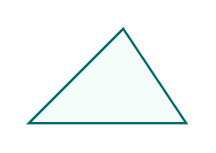
\begin{tikzpicture}[scale=1, baseline=(current bounding box.center)]
      \coordinate (A) at (0,0); \coordinate (B) at (2.0,0); \coordinate (C) at (1.2,1.2);
      \fill[brandTealBg] (A) -- (B) -- (C) -- cycle;
      \draw[thick, brandNavy] (A) -- (B) -- (C) -- cycle;
    \end{tikzpicture} &
    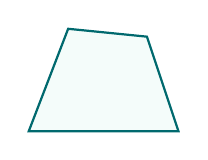
\begin{tikzpicture}[scale=1, baseline=(current bounding box.center)]
      \coordinate (A) at (0,0); \coordinate (B) at (1.9,0); \coordinate (C) at (1.5,1.2); \coordinate (D) at (0.5,1.3);
      \fill[brandTealBg] (A) -- (B) -- (C) -- (D) -- cycle;
      \draw[thick, brandNavy] (A) -- (B) -- (C) -- (D) -- cycle;
    \end{tikzpicture} &
    
\begin{tikzpicture}[scale=1, baseline=(current bounding box.center)]
      \coordinate (A) at (0.3,1.3); \coordinate (B) at (1.7,1.3); \coordinate (C) at (1.5,0.4); \coordinate (D) at (1.0,0.0); \coordinate (E) at (0.1,0.5);
      \fill[brandTealBg] (A) -- (B) -- (C) -- (D) -- (E) -- cycle;
      \draw[thick, brandNavy] (A) -- (B) -- (C) -- (D) -- (E) -- cycle;
    \end{tikzpicture} &
    
\begin{tikzpicture}[scale=1, baseline=(current bounding box.center)]
      \coordinate (A) at (0.4,1.1); \coordinate (B) at (1.6,1.1); \coordinate (C) at (2.0,0.55); \coordinate (D) at (1.6,0.0); \coordinate (E) at (0.4,0.0); \coordinate (F) at (0.0,0.55);
      \fill[brandTealBg] (A) -- (B) -- (C) -- (D) -- (E) -- cycle;
      \draw[thick, brandNavy] (A) -- (B) -- (C) -- (D) -- (E) -- (F) -- cycle;
    \end{tikzpicture} \\
    \hline
    \textbf{ចំនួនជ្រុង} & $3$ & $4$ & $5$ & $6$ \\
    \hline
  \end{tabular}
\end{center}

\vspace{2pt}

% Problem 1
\noindent
\begin{minipage}{\linewidth}
  \exhead{1} រាប់ចំនួនមុំ និងចំនួនជ្រុងនៃពហុកោណតាមរូបខាងក្រោម ៖
  \begin{center}
    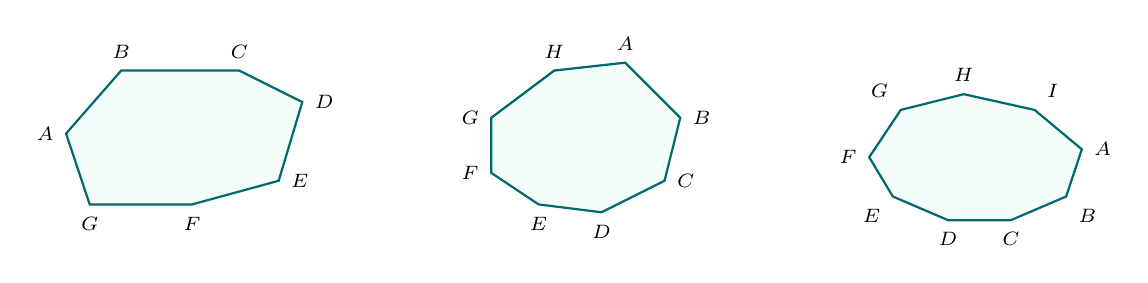
\begin{tikzpicture}[scale=1]
      % Figure 1: Heptagon (7 sides) ABCDEFG
      \begin{scope}[xshift=-5.0cm]
        \coordinate (A) at (-1.5, 0.3);
        \coordinate (B) at (-0.8, 1.1);
        \coordinate (C) at (0.7, 1.1);
        \coordinate (D) at (1.5, 0.7);
        \coordinate (E) at (1.2, -0.3);
        \coordinate (F) at (0.1, -0.6);
        \coordinate (G) at (-1.2, -0.6);
        
        \fill[brandTealBg] (A) -- (B) -- (C) -- (D) -- (E) -- (F) -- (G) -- cycle;
        \draw[thick, brandNavy] (A) -- (B) -- (C) -- (D) -- (E) -- (F) -- (G) -- cycle;
        
        \node[left=1pt, font=\fontsize{7}{7}\selectfont] at (A) {$A$};
        \node[above=1pt, font=\fontsize{7}{7}\selectfont] at (B) {$B$};
        \node[above=1pt, font=\fontsize{7}{7}\selectfont] at (C) {$C$};
        \node[right=1pt, font=\fontsize{7}{7}\selectfont] at (D) {$D$};
        \node[right=1pt, font=\fontsize{7}{7}\selectfont] at (E) {$E$};
        \node[below=1pt, font=\fontsize{7}{7}\selectfont] at (F) {$F$};
        \node[below=1pt, font=\fontsize{7}{7}\selectfont] at (G) {$G$};
      \end{scope}
      
      % Figure 2: Octagon (8 sides) ABCDEFGH
      \begin{scope}[xshift=0cm]
        \coordinate (A) at (0.6, 1.2);
        \coordinate (B) at (1.3, 0.5);
        \coordinate (C) at (1.1, -0.3);
        \coordinate (D) at (0.3, -0.7);
        \coordinate (E) at (-0.5, -0.6);
        \coordinate (F) at (-1.1, -0.2);
        \coordinate (G) at (-1.1, 0.5);
        \coordinate (H) at (-0.3, 1.1);
        
        \fill[brandTealBg] (A) -- (B) -- (C) -- (D) -- (E) -- (F) -- (G) -- (H) -- cycle;
        \draw[thick, brandNavy] (A) -- (B) -- (C) -- (D) -- (E) -- (F) -- (G) -- (H) -- cycle;
        
        \node[above=1pt, font=\fontsize{7}{7}\selectfont] at (A) {$A$};
        \node[right=1pt, font=\fontsize{7}{7}\selectfont] at (B) {$B$};
        \node[right=1pt, font=\fontsize{7}{7}\selectfont] at (C) {$C$};
        \node[below=1pt, font=\fontsize{7}{7}\selectfont] at (D) {$D$};
        \node[below=1pt, font=\fontsize{7}{7}\selectfont] at (E) {$E$};
        \node[left=1pt, font=\fontsize{7}{7}\selectfont] at (F) {$F$};
        \node[left=1pt, font=\fontsize{7}{7}\selectfont] at (G) {$G$};
        \node[above=1pt, font=\fontsize{7}{7}\selectfont] at (H) {$H$};
      \end{scope}
      
      % Figure 3: Nonagon (9 sides) ABCDEFGHI
      \begin{scope}[xshift=5.0cm]
        \coordinate (A) at (1.4, 0.1);
        \coordinate (B) at (1.2, -0.5);
        \coordinate (C) at (0.5, -0.8);
        \coordinate (D) at (-0.3, -0.8);
        \coordinate (E) at (-1.0, -0.5);
        \coordinate (F) at (-1.3, 0.0);
        \coordinate (G) at (-0.9, 0.6);
        \coordinate (H) at (-0.1, 0.8);
        \coordinate (I) at (0.8, 0.6);
        
        \fill[brandTealBg] (A) -- (B) -- (C) -- (D) -- (E) -- (F) -- (G) -- (H) -- (I) -- cycle;
        \draw[thick, brandNavy] (A) -- (B) -- (C) -- (D) -- (E) -- (F) -- (G) -- (H) -- (I) -- cycle;
        
        \node[right=1pt, font=\fontsize{7}{7}\selectfont] at (A) {$A$};
        \node[below right=1pt, font=\fontsize{7}{7}\selectfont] at (B) {$B$};
        \node[below=1pt, font=\fontsize{7}{7}\selectfont] at (C) {$C$};
        \node[below=1pt, font=\fontsize{7}{7}\selectfont] at (D) {$D$};
        \node[below left=1pt, font=\fontsize{7}{7}\selectfont] at (E) {$E$};
        \node[left=1pt, font=\fontsize{7}{7}\selectfont] at (F) {$F$};
        \node[above left=1pt, font=\fontsize{7}{7}\selectfont] at (G) {$G$};
        \node[above=1pt, font=\fontsize{7}{7}\selectfont] at (H) {$H$};
        \node[above right=1pt, font=\fontsize{7}{7}\selectfont] at (I) {$I$};
      \end{scope}
    \end{tikzpicture}
  \end{center}
\end{minipage}

\vspace{2pt}

\begin{multicols}{2}

% Problem 2
\noindent
\begin{minipage}{\linewidth}
  \exhead{2} ចូរប្រាប់ចំនួនជ្រុង និងគណនាចំនួនអង្កត់ទ្រូងសរុបនៃពហុកោណខាងក្រោម ៖\\
  \khlabel{ក} បញ្ចកោណ \hfill \khlabel{ខ} ឆកោណ\\
  \khlabel{គ} អដ្ឋកោណ \hfill \khlabel{ឃ} ទសកោណ
  \begin{center}
    \begin{tikzpicture}[scale=1]
      \foreach \i in {0,1,2,3,4,5} {
        \coordinate (V\i) at ({60*\i}:1.2);
      }
      \fill[brandTealBg] (V0) -- (V1) -- (V2) -- (V3) -- (V4) -- (V5) -- cycle;
      \draw[thick, brandNavy] (V0) -- (V1) -- (V2) -- (V3) -- (V4) -- (V5) -- cycle;
      \foreach \i in {0,1,2,3,4,5} {
        \fill[brandNavy] (V\i) circle (1.4pt);
      }
      \draw[dashed, brandCrimson, line width=0.6pt] (V0) -- (V2);
      \draw[dashed, brandCrimson, line width=0.6pt] (V0) -- (V3);
      \draw[dashed, brandCrimson, line width=0.6pt] (V0) -- (V4);
      \node[below=2pt, font=\fontsize{7.5}{7.5}\selectfont\kml, color=brandNavy] at (0, -1.3) {ឆកោណ ($d = 3, D = 9$)};
    \end{tikzpicture}
  \end{center}
\end{minipage}

\vspace{6pt}
% Problem 3
\noindent
\begin{minipage}{\linewidth}
  \exhead{3} គេមានពហុកោណមួយចំនួនដូចខាងក្រោម ៖\\
  \khlabel{ក} ពហុកោណមួយមាន $12$ ជ្រុង ។ រកចំនួនអង្កត់ទ្រូងគូសចេញពីកំពូលមួយ និងចំនួនអង្កត់ទ្រូងសរុប ។\\
  \khlabel{ខ} គេអាចគូសអង្កត់ទ្រូងចេញពីកំពូលមួយនៃពហុកោណមួយបានចំនួន $6$ អង្កត់ទ្រូង ។ រកចំនួនជ្រុង និងចំនួនអង្កត់ទ្រូងសរុប 
\end{minipage}

\columnbreak

% Problem 4
\noindent
\begin{minipage}{\linewidth}
  \exhead{4} ពហុកោណមួយមានអង្កត់ទ្រូងសរុបចំនួន $20$ ។\\
  \khlabel{ក} តើពហុកោណនោះមានប៉ុន្មានជ្រុង?\\
  \khlabel{ខ} ចូរប្រាប់ឈ្មោះពហុកោណនោះ ។
  \begin{center}
    \begin{tikzpicture}[scale=1]
      \foreach \i in {0,1,...,7} {
        \coordinate (P\i) at ({45*\i}:1.25);
      }
      \fill[brandTealBg] (P0) \foreach \i in {1,...,7} { -- (P\i) } -- cycle;
      \draw[thick, brandNavy] (P0) \foreach \i in {1,...,7} { -- (P\i) } -- cycle;
      \foreach \i in {0,1,...,7} {
        \fill[brandNavy] (P\i) circle (1.4pt);
      }
      \draw[dashed, brandCrimson, line width=0.6pt] (P0) -- (P3);
      \draw[dashed, brandCrimson, line width=0.6pt] (P0) -- (P4);
      \draw[dashed, brandCrimson, line width=0.6pt] (P0) -- (P5);
      \node[below=2pt, font=\fontsize{7.5}{7.5}\selectfont\kml, color=brandNavy] at (0, -1.35) {អដ្ឋកោណ ($D = 20$)};
    \end{tikzpicture}
  \end{center}
\end{minipage}

\vspace{3pt}
% Problem 5
\noindent
\begin{minipage}{\linewidth}
  \exhead{5} ពហុកោណមួយមានអង្កត់ទ្រូងសរុបច្រើនជាងចំនួនជ្រុងរបស់វាចំនួន $12$ ។\\
  \khlabel{ក} ចូរគណនាចំនួនជ្រុង $n$ នៃពហុកោណនោះ ។\\
  \khlabel{ខ} តើគេអាចគូសអង្កត់ទ្រូងចេញពីកំពូលមួយបានប៉ុន្មាន?
\end{minipage}

\end{multicols}

% =========================================================================
% ផ្នែកទី ២ ៖ ផលបូករង្វាស់មុំក្នុងនៃពហុកោណ
% =========================================================================
\khsection{២}{ផលបូករង្វាស់មុំក្នុងនៃពហុកោណ}

\begin{khboxorange}
  \begin{minipage}[c]{0.65\textwidth}
    \begin{itemize}[leftmargin=12pt, itemsep=3pt, topsep=1pt, parsep=0pt]
      \item[\color{brandNavy}\ding{228}] \textbf{ទ្រឹស្ដីបទ ៖} ផលបូករង្វាស់មុំក្នុងនៃពហុកោណប៉ោងមួយដែលមាន $n$ ជ្រុង ($n \ge 3$) គឺស្មើនឹង $(n - 2)$ ដងនៃ $180^\circ$ ៖
      \begin{equation*}
        \koreahl{$S_n = (n - 2) \times 180^\circ$}
      \end{equation*}
      \item[\color{brandCrimson}\ding{228}] \textbf{សម្រាយបញ្ជាក់ ៖}
      តាមកំពូលមួយនៃពហុកោណប៉ោង $n$ ជ្រុង គេអាចគូសអង្កត់ទ្រូងបំបែកពហុកោណជា $(n - 2)$ ត្រីកោណ ។\\
      ដោយផលបូករង្វាស់មុំក្នុងនៃត្រីកោណនីមួយៗស្មើ $180^\circ$ ដូចនេះផលបូករង្វាស់មុំក្នុងសរុបនៃពហុកោណគឺ ៖
      \begin{equation*}
        S_n = (n - 2) \times 180^\circ
      \end{equation*}
    \end{itemize}
  \end{minipage}\hfill
  \begin{minipage}[c]{0.33\textwidth}
    \centering
    \begin{tikzpicture}[scale=1]
      % Hexagon showing triangulation from vertex A_1
      \coordinate (A1) at (0, 0);
      \coordinate (A2) at (1.8, -0.4);
      \coordinate (A3) at (3.0, 0.9);
      \coordinate (A4) at (2.4, 2.4);
      \coordinate (A5) at (0.9, 2.7);
      \coordinate (A6) at (-0.6, 1.4);
      
      \fill[brandTealBg] (A1) -- (A2) -- (A3) -- (A4) -- (A5) -- (A6) -- cycle;
      \draw[thick, brandNavy] (A1) -- (A2) -- (A3) -- (A4) -- (A5) -- (A6) -- cycle;
      
      % Diagonals from A1
      \draw[dashed, brandCrimson, line width=0.7pt] (A1) -- (A3);
      \draw[dashed, brandCrimson, line width=0.7pt] (A1) -- (A4);
      \draw[dashed, brandCrimson, line width=0.7pt] (A1) -- (A5);
      
      % Label Triangles
      \node[font=\fontsize{7}{7}\selectfont\bfseries, color=brandCrimson] at (1.6, 0.2) {$T_1$};
      \node[font=\fontsize{7}{7}\selectfont\bfseries, color=brandCrimson] at (1.8, 1.1) {$T_2$};
      \node[font=\fontsize{7}{7}\selectfont\bfseries, color=brandCrimson] at (1.2, 1.7) {$T_3$};
      \node[font=\fontsize{7}{7}\selectfont\bfseries, color=brandCrimson] at (0.1, 1.4) {$T_4$};
      
      % Vertices
      \foreach \p/\n/\pos in {A1/A_1/below left, A2/A_2/below, A3/A_3/right, A4/A_4/above right, A5/A_5/above, A6/A_6/left} {
        \fill[brandNavy] (\p) circle (1.5pt);
        \node[\pos=1pt, font=\fontsize{7}{7}\selectfont] at (\p) {$\n$};
      }
      \node[below=2pt, font=\fontsize{7.5}{7.5}\selectfont\kml, color=brandNavy] at (1.4, -0.6) {ឆកោណ ($n=6 \implies 4$ ត្រីកោណ)};
    \end{tikzpicture}
  \end{minipage}
\end{khboxorange}

\vspace{3pt}

\begin{multicols}{2}

% Problem 6
\noindent
\begin{minipage}{\linewidth}
  \exhead{6} គណនាផលបូករង្វាស់មុំក្នុងនៃពហុកោណខាងក្រោម ៖\\
  \khlabel{ក} បញ្ចកោណ ($n = 5$)\\
  \khlabel{ខ} អដ្ឋកោណ ($n = 8$)\\
  \khlabel{គ} ពហុកោណមាន $14$ ជ្រុង\\
  \khlabel{ឃ} ពហុកោណមាន $20$ ជ្រុង
\end{minipage}

\vspace{6pt}
% Problem 7
\noindent
\begin{minipage}{\linewidth}
  \exhead{7} រកចំនួនជ្រុង $n$ នៃពហុកោណប៉ោងមួយ បើគេដឹងថាផលបូករង្វាស់មុំក្នុងរបស់វាស្មើនឹង ៖\\
  \khlabel{ក} $1080^\circ$\hfill \khlabel{ខ} $1440^\circ$\\
  \khlabel{គ} $1800^\circ$\hfill \khlabel{ឃ} $2340^\circ$
\end{minipage}

\vspace{6pt}
% Problem 8
\noindent
\begin{minipage}{\linewidth}
  \exhead{8} គេមានពហុកោណប៉ោងមួយដែលមានផលបូករង្វាស់មុំក្នុងស្មើនឹង $1260^\circ$ ៖\\
  \khlabel{ក} រកចំនួនជ្រុង $n$ នៃពហុកោណនោះ ។\\
  \khlabel{ខ} គណនាចំនួនអង្កត់ទ្រូងសរុបនៃពហុកោណនោះ ។
\end{minipage}

\columnbreak

% Problem 9
\noindent
\begin{minipage}{\linewidth}
  \exhead{9} គណនាតម្លៃនៃ $x$ ក្នុងរូបពហុកោណខាងក្រោម ៖
  \begin{center}
    \begin{tikzpicture}[scale=1]
      \coordinate (A) at (0, 0);
      \coordinate (B) at (3.2, 0);
      \coordinate (C) at (2.6, 2.0);
      \coordinate (D) at (1.0, 2.3);
      \coordinate (E) at (-0.6, 1.1);
      
      \fill[brandTealBg] (A) -- (B) -- (C) -- (D) -- (E) -- cycle;
      \draw[thick, brandNavy] (A) -- (B) -- (C) -- (D) -- (E) -- cycle;
      
      \node[above right=1pt, font=\fontsize{7.5}{7.5}\selectfont] at (A) {$110^\circ$};
      \node[above left=1pt, font=\fontsize{7.5}{7.5}\selectfont] at (B) {$100^\circ$};
      \node[below left=1pt, font=\fontsize{7.5}{7.5}\selectfont] at (C) {$125^\circ$};
      \node[below=2pt, font=\fontsize{7.5}{7.5}\selectfont] at (D) {$95^\circ$};
      \node[right=2pt, font=\fontsize{8}{8}\selectfont\bfseries, color=brandCrimson] at (E) {$x$};
      
      \node[below=2pt, font=\fontsize{7.5}{7.5}\selectfont\kml, color=gray!80] at (1.3, -0.2) {បញ្ចកោណ ($5$ ជ្រុង)};
    \end{tikzpicture}
  \end{center}
\end{minipage}

\vspace{3pt}
% Problem 10
\noindent
\begin{minipage}{\linewidth}
  \exhead{10} ក្នុងចតុកោណមួយ រង្វាស់មុំក្នុងទាំងបួនមានផលធៀបជា $2 : 3 : 4 : 6$ (ដូចរូប) ។\\
  ចូរគណនារង្វាស់មុំក្នុងនីមួយៗនៃចតុកោណនោះ ។
  \begin{center}
    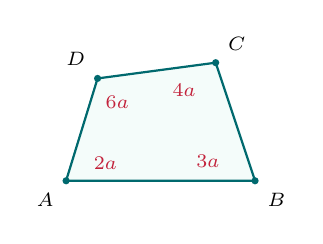
\begin{tikzpicture}[scale=1]
      \coordinate (A) at (0, 0);
      \coordinate (B) at (2.4, 0);
      \coordinate (C) at (1.9, 1.5);
      \coordinate (D) at (0.4, 1.3);
      \fill[brandTealBg] (A) -- (B) -- (C) -- (D) -- cycle;
      \draw[thick, brandNavy] (A) -- (B) -- (C) -- (D) -- cycle;
      \foreach \p/\n/\pos in {A/A/below left, B/B/below right, C/C/above right, D/D/above left} {
        \fill[brandNavy] (\p) circle (1.3pt);
        \node[\pos=1pt, font=\fontsize{7}{7}\selectfont] at (\p) {$\n$};
      }
      \node[font=\fontsize{7}{7}\selectfont\bfseries, color=brandCrimson] at (0.5, 0.22) {$2a$};
      \node[font=\fontsize{7}{7}\selectfont\bfseries, color=brandCrimson] at (1.8, 0.25) {$3a$};
      \node[font=\fontsize{7}{7}\selectfont\bfseries, color=brandCrimson] at (1.5, 1.15) {$4a$};
      \node[font=\fontsize{7}{7}\selectfont\bfseries, color=brandCrimson] at (0.65, 1.0) {$6a$};
    \end{tikzpicture}
  \end{center}
\end{minipage}

\vspace{3pt}
% Problem 11
\noindent
\begin{minipage}{\linewidth}
  \exhead{11} គណនាតម្លៃនៃ $x$ ក្នុងរូបឆកោណខាងក្រោម ៖
  \begin{center}
    \begin{tikzpicture}[scale=1]
      \coordinate (A) at (0, 0);
      \coordinate (B) at (2.2, 0);
      \coordinate (C) at (2.8, 1.2);
      \coordinate (D) at (2.0, 2.2);
      \coordinate (E) at (0.5, 2.2);
      \coordinate (F) at (-0.5, 1.0);
      
      \fill[brandTealBg] (A) -- (B) -- (C) -- (D) -- (E) -- (F) -- cycle;
      \draw[thick, brandNavy] (A) -- (B) -- (C) -- (D) -- (E) -- (F) -- cycle;
      
      \node[font=\fontsize{6.5}{6.5}\selectfont] at (0.25, 0.2) {$120^\circ$};
      \node[font=\fontsize{6.5}{6.5}\selectfont] at (1.95, 0.2) {$130^\circ$};
      \node[font=\fontsize{6.5}{6.5}\selectfont] at (2.55, 1.2) {$115^\circ$};
      \node[font=\fontsize{6.5}{6.5}\selectfont] at (1.85, 1.95) {$140^\circ$};
      \node[font=\fontsize{6.5}{6.5}\selectfont] at (0.65, 1.95) {$105^\circ$};
      \node[font=\fontsize{7.5}{7.5}\selectfont\bfseries, color=brandCrimson] at (-0.25, 1.0) {$x$};
      
      \node[below=2pt, font=\fontsize{7.5}{7.5}\selectfont\kml, color=gray!80] at (1.1, -0.15) {ឆកោណ ($6$ ជ្រុង, $S_6 = 720^\circ$)};
    \end{tikzpicture}
  \end{center}
\end{minipage}

\end{multicols}

% =========================================================================
% ផ្នែកទី ៣ ៖ ផលបូករង្វាស់មុំក្រៅនៃពហុកោណ
% =========================================================================
\khsection{៣}{ផលបូករង្វាស់មុំក្រៅនៃពហុកោណ}

\begin{khboxorange}
  \begin{minipage}[c]{0.63\textwidth}
    \begin{itemize}[leftmargin=12pt, itemsep=2.5pt, topsep=1pt, parsep=0pt]
      \item[\color{brandNavy}\ding{228}] \textbf{និយមន័យ ៖} \textbf{មុំក្រៅ} នៃពហុកោណ គឺជាមុំដែលផ្គុំឡើងរវាង \textbf{ជ្រុងមួយ} និង \textbf{បន្លាយនៃជ្រុងជាប់វា} (នៅត្រង់កំពូលនីមួយៗ) ។
      \item[\color{brandNavy}\ding{228}] \textbf{ទ្រឹស្ដីបទ ៖} ផលបូករង្វាស់មុំក្រៅ (គិតមួយនៅកំពូលនីមួយៗ) នៃពហុកោណប៉ោងគ្រប់ប្រភេទ មានរង្វាស់ស្មើនឹង \koreahl{$360^\circ$} ជានិច្ច ៖
      \begin{equation*}
        \koreahl{$\sum \text{មុំក្រៅ} = 360^\circ$}
      \end{equation*}
      \item[\color{brandCrimson}\ding{228}] \textbf{សម្រាយបញ្ជាក់ ៖}
      នៅកំពូលនីមួយៗ មុំក្នុង និងមុំក្រៅជាមុំជាប់បំពេញ (ផលបូកស្មើ $180^\circ$) ។\\
      ពហុកោណមាន $n$ កំពូល នាំឱ្យ ៖
      \begin{align*}
        (\text{ផលបូកមុំក្នុង}) + (\text{ផលបូកមុំក្រៅ}) &= n \times 180^\circ \\
        (\text{ផលបូកមុំក្រៅ}) &= n \times 180^\circ - (n - 2) \times 180^\circ \\
        &= 180^\circ \times [n - (n - 2)] = 2 \times 180^\circ = \mathbf{360^\circ}
      \end{align*}
    \end{itemize}
  \end{minipage}\hfill
  \begin{minipage}[c]{0.36\textwidth}
    \centering
    \begin{tikzpicture}[scale=1]
      % Vertices of convex pentagon (counter-clockwise)
      \coordinate (A) at (0.0, 1.25);
      \coordinate (B) at (-1.15, 0.45);
      \coordinate (C) at (-0.75, -0.90);
      \coordinate (D) at (0.75, -0.90);
      \coordinate (E) at (1.15, 0.45);
      
      % Interior fill & polygon outline
      \fill[brandTealBg] (A) -- (B) -- (C) -- (D) -- (E) -- cycle;
      \draw[thick, brandNavy] (A) -- (B) -- (C) -- (D) -- (E) -- cycle;
      
      % Outer cyclic extensions (extending side outward in cyclic direction)
      \coordinate (XA) at ($(E)!1.7!(A)$);
      \coordinate (XB) at ($(A)!1.65!(B)$);
      \coordinate (XC) at ($(B)!1.65!(C)$);
      \coordinate (XD) at ($(C)!1.65!(D)$);
      \coordinate (XE) at ($(D)!1.65!(E)$);
      
      \draw[thick, brandCrimson, ->, >=stealth] (A) -- (XA);
      \draw[thick, brandCrimson, ->, >=stealth] (B) -- (XB);
      \draw[thick, brandCrimson, ->, >=stealth] (C) -- (XC);
      \draw[thick, brandCrimson, ->, >=stealth] (D) -- (XD);
      \draw[thick, brandCrimson, ->, >=stealth] (E) -- (XE);
      
      % Exterior angle arcs (counter-clockwise from extended ray to next edge)
      \pic [draw, brandCrimson, thick, fill=brandCrimson!25, angle radius=0.45cm] {angle = XA--A--B};
      \pic [draw, brandCrimson, thick, fill=brandCrimson!20, angle radius=0.36cm] {angle = XB--B--C};
      \pic [draw, brandCrimson, thick, fill=brandCrimson!20, angle radius=0.36cm] {angle = XC--C--D};
      \pic [draw, brandCrimson, thick, fill=brandCrimson!20, angle radius=0.36cm] {angle = XD--D--E};
      \pic [draw, brandCrimson, thick, fill=brandCrimson!20, angle radius=0.36cm] {angle = XE--E--A};
      
      % Interior angle arc at A showing supplementary angle
      \pic [draw, brandNavy, thick, fill=brandNavy!18, angle radius=0.38cm] {angle = B--A--E};
      
      % Vertex dots
      \foreach \p in {A,B,C,D,E} {
        \fill[brandNavy] (\p) circle (1.2pt);
      }

      % Annotations pointing clearly with precision (no crossing lines):
      % 1. Exterior Angle e1 (points horizontally into the exact center of exterior angle arc)
      \draw[thick, brandCrimson, ->, >=stealth] (-1.35, 1.25) node[left=-1pt, font=\fontsize{7.5}{7.5}\selectfont\kml, color=brandCrimson] {មុំក្រៅ ($e_1$)} -- (-0.48, 1.25);

      % 2. Side extension (points from top-left directly to the extension ray)
      \draw[thick, gray!75, ->, >=stealth] (-1.35, 2.05) node[left=-1pt, font=\fontsize{6.5}{6.5}\selectfont\kml, color=gray!80] {បន្លាយជ្រុង} to[out=0, in=135] (-0.45, 1.56);

      % 3. Interior Angle i1 (points from top-right directly into interior angle arc)
      \draw[thick, brandNavy, ->, >=stealth] (1.3, 1.35) node[right=-1pt, font=\fontsize{7.5}{7.5}\selectfont\kml, color=brandNavy] {មុំក្នុង ($i_1$)} to[out=180, in=30] (0.08, 0.96);

      % Labels for remaining exterior angles
      \node[above left=1pt, font=\fontsize{7.5}{7.5}\selectfont\bfseries, color=brandCrimson] at ($(B)!0.6!(XB)$) {$e_2$};
      \node[below left=1pt, font=\fontsize{7.5}{7.5}\selectfont\bfseries, color=brandCrimson] at ($(C)!0.6!(XC)$) {$e_3$};
      \node[below right=1pt, font=\fontsize{7.5}{7.5}\selectfont\bfseries, color=brandCrimson] at ($(D)!0.6!(XD)$) {$e_4$};
      \node[right=1pt, font=\fontsize{7.5}{7.5}\selectfont\bfseries, color=brandCrimson] at ($(E)!0.6!(XE)$) {$e_5$};
      
      \node[below=2pt, font=\fontsize{10}{7}\selectfont\kml\bfseries, color=brandCrimson] at (0, -1.85) {$e_1+e_2+e_3+e_4+e_5=360^\circ$};
      \node[below=15pt, font=\fontsize{10}{6.5}\selectfont\kml, color=brandNavy] at (0, -1.85) {$i_1+e_1=180^\circ$ (មុំជាប់បំពេញ)};
    \end{tikzpicture}
  \end{minipage}
\end{khboxorange}

\vspace{3pt}

\begin{multicols}{2}

% Problem 12
\noindent
\begin{minipage}{\linewidth}
  \exhead{12} តាមរូបខាងក្រោម ចូរគណនាតម្លៃនៃ $x$ ៖
  \begin{center}
    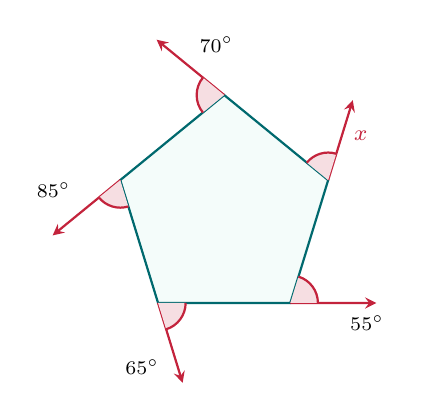
\begin{tikzpicture}[scale=1.2]
      \coordinate (A) at (0, 1.35);
      \coordinate (B) at (-1.1, 0.45);
      \coordinate (C) at (-0.7, -0.85);
      \coordinate (D) at (0.7, -0.85);
      \coordinate (E) at (1.1, 0.45);
      
      \fill[brandTealBg] (A) -- (B) -- (C) -- (D) -- (E) -- cycle;
      \draw[thick, brandNavy] (A) -- (B) -- (C) -- (D) -- (E) -- cycle;
      
      \coordinate (XA) at ($(E)!1.65!(A)$);
      \coordinate (XB) at ($(A)!1.65!(B)$);
      \coordinate (XC) at ($(B)!1.65!(C)$);
      \coordinate (XD) at ($(C)!1.65!(D)$);
      \coordinate (XE) at ($(D)!1.65!(E)$);
      
      \draw[thick, brandCrimson, ->, >=stealth] (A) -- (XA);
      \draw[thick, brandCrimson, ->, >=stealth] (B) -- (XB);
      \draw[thick, brandCrimson, ->, >=stealth] (C) -- (XC);
      \draw[thick, brandCrimson, ->, >=stealth] (D) -- (XD);
      \draw[thick, brandCrimson, ->, >=stealth] (E) -- (XE);
      
      \pic [draw, brandCrimson, thick, fill=brandCrimson!15, angle radius=0.35cm] {angle = XA--A--B};
      \pic [draw, brandCrimson, thick, fill=brandCrimson!15, angle radius=0.35cm] {angle = XB--B--C};
      \pic [draw, brandCrimson, thick, fill=brandCrimson!15, angle radius=0.35cm] {angle = XC--C--D};
      \pic [draw, brandCrimson, thick, fill=brandCrimson!15, angle radius=0.35cm] {angle = XD--D--E};
      \pic [draw, brandCrimson, thick, fill=brandCrimson!15, angle radius=0.35cm] {angle = XE--E--A};
      
      \node[above right=1pt, font=\fontsize{7.5}{7.5}\selectfont] at ($(A)!0.55!(XA)$) {$70^\circ$};
      \node[above left=1pt, font=\fontsize{7.5}{7.5}\selectfont] at ($(B)!0.55!(XB)$) {$85^\circ$};
      \node[below left=1pt, font=\fontsize{7.5}{7.5}\selectfont] at ($(C)!0.55!(XC)$) {$65^\circ$};
      \node[below right=1pt, font=\fontsize{7.5}{7.5}\selectfont] at ($(D)!0.55!(XD)$) {$55^\circ$};
      \node[right=1pt, font=\fontsize{8}{8}\selectfont\bfseries, color=brandCrimson] at ($(E)!0.55!(XE)$) {$x$};
    \end{tikzpicture}
  \end{center}
\end{minipage}

\vspace{3pt}
% Problem 13
\noindent
\begin{minipage}{\linewidth}
  \exhead{13} គណនាតម្លៃនៃ $y$ ក្នុងរូបចតុកោណខាងក្រោម ៖
  \begin{center}
    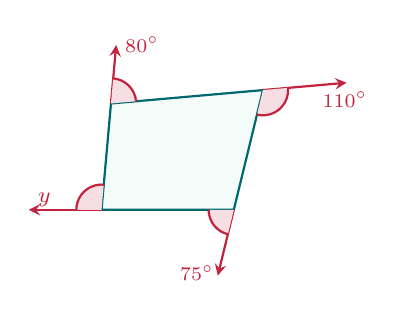
\begin{tikzpicture}[scale=1]
      \coordinate (D) at (0, 0);
      \coordinate (A) at (0.12, 1.35);
      \coordinate (B) at (2.05, 1.52);
      \coordinate (C) at (1.68, 0);

      % Polygon Fill and Outline
      \fill[brandTealBg] (A) -- (B) -- (C) -- (D) -- cycle;
      \draw[thick, brandNavy] (A) -- (B) -- (C) -- (D) -- cycle;

      % Extension coordinates
      \coordinate (XA) at ($(D)!1.55!(A)$);
      \coordinate (XB) at ($(A)!1.55!(B)$);
      \coordinate (XC) at ($(B)!1.55!(C)$);
      \coordinate (XD) at ($(C)!1.55!(D)$);

      % Extension Rays with Arrows
      \draw[thick, brandCrimson, ->, >=stealth] (A) -- (XA);
      \draw[thick, brandCrimson, ->, >=stealth] (B) -- (XB);
      \draw[thick, brandCrimson, ->, >=stealth] (C) -- (XC);
      \draw[thick, brandCrimson, ->, >=stealth] (D) -- (XD);

      % Angle Arcs
      \pic [draw, brandCrimson, thick, fill=brandCrimson!15, angle radius=0.32cm] {angle = B--A--XA};
      \pic [draw, brandCrimson, thick, fill=brandCrimson!15, angle radius=0.32cm] {angle = C--B--XB};
      \pic [draw, brandCrimson, thick, fill=brandCrimson!15, angle radius=0.32cm] {angle = D--C--XC};
      \pic [draw, brandCrimson, thick, fill=brandCrimson!15, angle radius=0.32cm] {angle = A--D--XD};

      % Angle Labels
      \node[above right=2pt, font=\fontsize{7.5}{7.5}\selectfont\bfseries, color=brandCrimson] at ($(A)!0.55!(XA)+(-0.05,0.05)$) {$80^\circ$};
      \node[below right=0pt, font=\fontsize{7.5}{7.5}\selectfont\bfseries, color=brandCrimson] at ($(B)!0.55!(XB)+(0.05,0.05)$) {$110^\circ$};
      \node[below left=2pt, font=\fontsize{7.5}{7.5}\selectfont\bfseries, color=brandCrimson] at ($(C)!0.55!(XC)+(0.05,-0.05)$) {$75^\circ$};
      \node[above left=-1pt, font=\fontsize{8.5}{8.5}\selectfont\bfseries, color=brandCrimson] at ($(D)!0.55!(XD)+(-0.05,-0.05)$) {$y$};
    \end{tikzpicture}
  \end{center}
\end{minipage}

\columnbreak

% Problem 14 (New Textbook Exercise from User Photo)
\noindent
\begin{minipage}{\linewidth}
  \exhead{14} ចូររកតម្លៃ $y$ តាមរូបនីមួយៗនៃពហុកោណខាងក្រោម ៖
  \begin{center}
    \begin{tikzpicture}[scale=1.2]
      % Figure (ក) - Quadrilateral
      \begin{scope}[xshift=0cm, yshift=0cm, scale=.7]
        \coordinate (Q1) at (0.4, 0);
        \coordinate (Q2) at (2.8, 0);
        \coordinate (Q3) at (3.5, 1.3);
        \coordinate (Q4) at (0.9, 1.8);
    
        \fill[brandTealBg] (Q1) -- (Q2) -- (Q3) -- (Q4) -- cycle;
        \draw[very thick, brandNavy] (Q1) -- (Q2) -- (Q3) -- (Q4) -- cycle;
    
        % Cyclic extensions counter-clockwise:
        \draw[thick, brandCrimson] (Q2) -- ($(Q1)!1.35!(Q2)$);
        \draw[thick, brandCrimson] (Q3) -- ($(Q2)!1.38!(Q3)$);
        \draw[thick, brandCrimson] (Q4) -- ($(Q3)!1.35!(Q4)$);
        \draw[thick, brandCrimson] (Q1) -- ($(Q4)!1.38!(Q1)$);
    
        % Labels:
        \node[above right=-1pt, font=\fontsize{7.5}{7.5}\selectfont\bfseries, color=brandNavy] at ($(Q2)+(0.12, 0.05)$) {$y$};
        \node[above left=-1pt, font=\fontsize{7.5}{7.5}\selectfont\bfseries, color=brandNavy] at ($(Q3)+(-0.05, 0.18)$) {$2y$};
        \node[below left=-1pt, font=\fontsize{7.5}{7.5}\selectfont\bfseries, color=brandNavy] at ($(Q4)+(-0.15, -0.05)$) {$y$};
        \node[below right=-1pt, font=\fontsize{7.5}{7.5}\selectfont\bfseries, color=brandNavy] at ($(Q1)+(-0.02, -0.15)$) {$2y$};
    
        \node[below=14pt, font=\fontsize{8}{8}\selectfont\bfseries] at (1.8, 0) {(ក)};
      \end{scope}
    
      % Figure (ខ) - Pentagon
      \begin{scope}[xshift=2.9cm, yshift=0cm, scale=0.7]
        \coordinate (P1) at (0.6, 0.15);
        \coordinate (P2) at (2.0, 0.45);
        \coordinate (P3) at (2.7, 1.35);
        \coordinate (P4) at (1.9, 1.95);
        \coordinate (P5) at (0.3, 0.95);
    
        \fill[brandTealBg] (P1) -- (P2) -- (P3) -- (P4) -- (P5) -- cycle;
        \draw[very thick, brandNavy] (P1) -- (P2) -- (P3) -- (P4) -- (P5) -- cycle;
    
        % Cyclic extensions counter-clockwise:
        \draw[thick, brandCrimson] (P2) -- ($(P3)!1.5!(P2)$);
        \draw[thick, brandCrimson] (P3) -- ($(P4)!1.5!(P3)$);
        \draw[thick, brandCrimson] (P4) -- ($(P5)!1.55!(P4)$);
        \draw[thick, brandCrimson] (P5) -- ($(P1)!1.55!(P5)$);
        \draw[thick, brandCrimson] (P1) -- ($(P2)!1.5!(P1)$);
    
        % Labels:
        \node[above left=-1pt, font=\fontsize{7}{7}\selectfont\bfseries, color=brandNavy] at ($(P1)+(-0.35, 0.05)$) {$70^\circ$};
        \node[below left=-1pt, font=\fontsize{7.5}{7.5}\selectfont\bfseries, color=brandNavy] at ($(P2)+(-0.25, -0.15)$) {$y$};
        \node[below right=-1pt, font=\fontsize{7.5}{7.5}\selectfont\bfseries, color=brandNavy] at ($(P3)+(0.08, -0.12)$) {$y$};
        \node[above right=-2pt, font=\fontsize{7.5}{7.5}\selectfont\bfseries, color=brandNavy] at ($(P4)+(0.12, 0.02)$) {$y$};
        \node[above right=-1pt, font=\fontsize{7}{7}\selectfont\bfseries, color=brandNavy] at ($(P5)+(-0.08, 0.18)$) {$80^\circ$};
    
        \node[below=14pt, font=\fontsize{8}{8}\selectfont\bfseries] at (1.5, 0) {(ខ)};
      \end{scope}
    
      % Figure (គ) - Heptagon
      \begin{scope}[xshift=6.0cm, yshift=0cm, scale=0.7]
        \coordinate (G) at (0.6, 0.15);
        \coordinate (A) at (1.8, 0.15);
        \coordinate (B) at (2.6, 0.95);
        \coordinate (C) at (2.2, 1.85);
        \coordinate (D) at (1.4, 2.25);
        \coordinate (E) at (0.5, 1.95);
        \coordinate (F) at (0.0, 1.15);
    
        \fill[brandTealBg] (G) -- (A) -- (B) -- (C) -- (D) -- (E) -- (F) -- cycle;
        \draw[very thick, brandNavy] (G) -- (A) -- (B) -- (C) -- (D) -- (E) -- (F) -- cycle;
    
        % Cyclic extensions counter-clockwise matching crop_heptagon.png:
        \draw[thick, brandCrimson] (A) -- ($(G)!1.45!(A)$);
        \draw[thick, brandCrimson] (B) -- ($(A)!1.45!(B)$);
        \draw[thick, brandCrimson] (C) -- ($(B)!1.45!(C)$);
        \draw[thick, brandCrimson] (D) -- ($(C)!1.55!(D)$);
        \draw[thick, brandCrimson] (E) -- ($(D)!1.55!(E)$);
        \draw[thick, brandCrimson] (F) -- ($(E)!1.55!(F)$);
        \draw[thick, brandCrimson] (G) -- ($(F)!1.45!(G)$);
    
        % Labels:
        \node[above right=-1pt, font=\fontsize{7}{7}\selectfont\bfseries, color=brandNavy] at ($(A)+(0.15, 0.08)$) {$2y$};
        \node[above right=-1pt, font=\fontsize{7}{7}\selectfont\bfseries, color=brandNavy] at ($(B)+(0.12, 0.12)$) {$3y$};
        \node[above left=-1pt, font=\fontsize{7}{7}\selectfont\bfseries, color=brandNavy] at ($(C)+(-0.02, 0.22)$) {$2y$};
        \node[above left=-1pt, font=\fontsize{7}{7}\selectfont\bfseries, color=brandNavy] at ($(D)+(-0.18, 0.06)$) {$2y$};
        \node[left=-1pt, font=\fontsize{7}{7}\selectfont\bfseries, color=brandNavy] at ($(E)+(-0.16, -0.05)$) {$2y$};
        \node[below left=-1pt, font=\fontsize{7}{7}\selectfont\bfseries, color=brandNavy] at ($(F)+(-0.12, -0.15)$) {$3y$};
        \node[below right=-1pt, font=\fontsize{7}{7}\selectfont\bfseries, color=brandNavy] at ($(G)+(0.12, -0.15)$) {$2y$};
    
        \node[below=14pt, font=\fontsize{8}{8}\selectfont\bfseries] at (1.3, 0) {(គ)};
      \end{scope}
    \end{tikzpicture}
  \end{center}
\end{minipage}

\vspace{2pt}
% Problem 15
\noindent
\begin{minipage}{\linewidth}
  \exhead{15} ផលបូករង្វាស់មុំក្នុងនៃពហុកោណមួយ ស្មើនឹង $3$ ដងនៃផលបូករង្វាស់មុំក្រៅរបស់វា ។\\
  \khlabel{ក} រកចំនួនជ្រុង $n$ នៃពហុកោណនោះ ។\\
  \khlabel{ខ} ប្រាប់ឈ្មោះនៃពហុកោណនោះ និងគណនាចំនួនអង្កត់ទ្រូងសរុប ។
\end{minipage}

\vspace{3pt}
% Problem 16
\noindent
\begin{minipage}{\linewidth}
  \exhead{16} រកចំនួនជ្រុងនៃពហុកោណមួយ បើដឹងថា ៖\\
  \khlabel{ក} ផលបូករង្វាស់មុំក្នុង ស្មើនឹងផលបូករង្វាស់មុំក្រៅរបស់វា ។\\
  \khlabel{ខ} ផលបូករង្វាស់មុំក្នុង ស្មើនឹង $2$ ដងនៃផលបូករង្វាស់មុំក្រៅរបស់វា ។
  \begin{center}
    \begin{tikzpicture}[scale=1]
      \coordinate (A) at (0,0); \coordinate (B) at (1.8,0); \coordinate (C) at (1.8,1.2); \coordinate (D) at (0,1.2);
      \fill[brandTealBg] (A) -- (B) -- (C) -- (D) -- cycle;
      \draw[thick, brandNavy] (A) -- (B) -- (C) -- (D) -- cycle;
      \draw[thick, brandCrimson, ->, >=stealth] (A) -- (2.4,0) node[right, font=\fontsize{6.5}{6.5}\selectfont] {$90^\circ$};
      \node[font=\fontsize{6.5}{6.5}\selectfont, color=brandNavy] at (0.3,0.3) {$90^\circ$};
      \node[below=2pt, font=\fontsize{7}{7}\selectfont\kml, color=brandNavy] at (0.9, -0.15) {$n = 4$ (ចតុកោណ, $S_4 = 360^\circ$)};
    \end{tikzpicture}
  \end{center}
\end{minipage}

\end{multicols}

% =========================================================================
% ផ្នែកទី ៤ ៖ ពហុកោណនិយ័ត
% =========================================================================
\khsection{៤}{ពហុកោណនិយ័ត (Regular Polygons)}

\begin{khboxorange}
  \begin{minipage}[c]{0.65\textwidth}
    \begin{itemize}[leftmargin=12pt, itemsep=2.5pt, topsep=1pt, parsep=0pt]
      \item[\color{brandNavy}\ding{228}] \textbf{និយមន័យ ៖} \textbf{ពហុកោណនិយ័ត} គឺជាពហុកោណដែលមានជ្រុងទាំងអស់មានប្រវែងស្មើគ្នា និងមុំទាំងអស់មានរង្វាស់ស្មើគ្នា ។
      \item[\color{brandCrimson}\ding{228}] ចំពោះពហុកោណនិយ័តដែលមាន $n$ ជ្រុង ($n \ge 3$) ៖
      \begin{itemize}[leftmargin=10pt, itemsep=2pt]
        \item រង្វាស់មុំក្នុងនីមួយៗ ៖ \koreahl{$\alpha = \dfrac{(n - 2) \times 180^\circ}{n}$}
        \item រង្វាស់មុំក្រៅនីមួយៗ ៖ \koreahl{$\beta = \dfrac{360^\circ}{n}$}
        \item ទំនាក់ទំនងមុំក្នុង និងមុំក្រៅ ៖ \koreahl{$\alpha + \beta = 180^\circ$}
      \end{itemize}
    \end{itemize}
  \end{minipage}\hfill
  \begin{minipage}[c]{0.33\textwidth}
    \centering
    \begin{tikzpicture}[scale=1]
      % Regular Hexagon
      \foreach \i in {0,1,2,3,4,5} {
        \coordinate (H\i) at ({60*\i}:1.35);
      }
      \fill[brandTealBg] (H0) -- (H1) -- (H2) -- (H3) -- (H4) -- (H5) -- cycle;
      \draw[thick, brandNavy] (H0) -- (H1) -- (H2) -- (H3) -- (H4) -- (H5) -- cycle;
      
      % Center and radii
      \coordinate (O) at (0,0);
      \fill[brandCrimson] (O) circle (1.5pt) node[below=1pt, font=\fontsize{7}{7}\selectfont] {$O$};
      \draw[dotted, thick, brandBlue] (O) -- (H0);
      \draw[dotted, thick, brandBlue] (O) -- (H1);
      
      % Mark tick marks on sides
      \foreach \i in {0,1,2,3,4,5} {
        \fill[brandNavy] (H\i) circle (1.3pt);
      }
      \draw[thick, brandCrimson] ($(H0)!0.5!(H1)+(-0.06,-0.04)$) -- ($(H0)!0.5!(H1)+(0.06,0.04)$);
      \draw[thick, brandCrimson] ($(H1)!0.5!(H2)+(-0.06,0.04)$) -- ($(H1)!0.5!(H2)+(0.06,-0.04)$);
      \draw[thick, brandCrimson] ($(H2)!0.5!(H3)+(-0.04,0.06)$) -- ($(H2)!0.5!(H3)+(0.04,-0.06)$);
      \draw[thick, brandCrimson] ($(H3)!0.5!(H4)+(-0.06,-0.04)$) -- ($(H3)!0.5!(H4)+(0.06,0.04)$);
      \draw[thick, brandCrimson] ($(H4)!0.5!(H5)+(-0.06,0.04)$) -- ($(H4)!0.5!(H5)+(0.06,-0.04)$);
      \draw[thick, brandCrimson] ($(H5)!0.5!(H0)+(-0.04,0.06)$) -- ($(H5)!0.5!(H0)+(0.04,-0.06)$);
      
      \node[below=2pt, font=\fontsize{7.5}{7.5}\selectfont\kml\bfseries, color=brandNavy] at (0, -1.5) {ឆកោណនិយ័ត ($\alpha=120^\circ$)};
    \end{tikzpicture}
  \end{minipage}
\end{khboxorange}

\vspace{2pt}
\noindent
\begin{center}
  \renewcommand{\arraystretch}{1.15}
  \fontsize{8}{8}\selectfont
  \begin{tabular}{|l|c|c|c|c|}
    \hline
    \rowcolor{brandNavy!15}
    \textbf{ពហុកោណនិយ័ត} & \textbf{ជ្រុង $n$} & \textbf{ផលបូកមុំក្នុង} & \textbf{មុំក្នុង $\alpha$} & \textbf{មុំក្រៅ $\beta$} \\
    \hline
    ត្រីកោណសម័ង្ស & $3$ & $180^\circ$ & $60^\circ$ & $120^\circ$ \\
    \hline
    ការ៉េ & $4$ & $360^\circ$ & $90^\circ$ & $90^\circ$ \\
    \hline
    បញ្ចកោណនិយ័ត & $5$ & $540^\circ$ & $108^\circ$ & $72^\circ$ \\
    \hline
    ឆកោណនិយ័ត & $6$ & $720^\circ$ & $120^\circ$ & $60^\circ$ \\
    \hline
    អដ្ឋកោណនិយ័ត & $8$ & $1080^\circ$ & $135^\circ$ & $45^\circ$ \\
    \hline
    ទសកោណនិយ័ត & $10$ & $1440^\circ$ & $144^\circ$ & $36^\circ$ \\
    \hline
    ទ្វាទសកោណនិយ័ត & $12$ & $1800^\circ$ & $150^\circ$ & $30^\circ$ \\
    \hline
  \end{tabular}
\end{center}

\vspace{2pt}

\begin{multicols}{2}

% Problem 17
\noindent
\begin{minipage}{\linewidth}
  \exhead{17} ចំពោះពហុកោណនិយ័តនីមួយៗខាងក្រោម ចូរគណនារង្វាស់មុំក្នុងមួយ ($\alpha$) និងមុំក្រៅមួយ ($\beta$) ៖\\
  \khlabel{ក} បញ្ចកោណនិយ័ត ($n = 5$)\\
  \khlabel{ខ} ឆកោណនិយ័ត ($n = 6$)\\
  \khlabel{គ} អដ្ឋកោណនិយ័ត ($n = 8$)\\
  \khlabel{ឃ} ទសកោណនិយ័ត ($n = 10$)
  \begin{center}
    \begin{tikzpicture}[scale=1]
      \foreach \i in {0,1,2,3,4} {
        \coordinate (R\i) at ({90+72*\i}:1.15);
      }
      \fill[brandTealBg] (R0) -- (R1) -- (R2) -- (R3) -- (R4) -- cycle;
      \draw[thick, brandNavy] (R0) -- (R1) -- (R2) -- (R3) -- (R4) -- cycle;
      %\draw[thick, brandCrimson, ->, >=stealth] (R2) -- ($(R3)!1.55!(R4)$) node[above right, font=\fontsize{7}{7}\selectfont] {$\beta$};
      \node[font=\fontsize{7}{7}\selectfont, color=brandNavy] at ($(R3)+(0.22, 0.1)$) {$\alpha$};
      \node[below=2pt, font=\fontsize{7.5}{7.5}\selectfont\kml, color=brandNavy] at (0, -1.25) {បញ្ចកោណ ($\alpha=108^\circ,\ \beta=72^\circ$)};
    \end{tikzpicture}
  \end{center}
\end{minipage}

\vspace{4pt}
% Problem 18
\noindent
\begin{minipage}{\linewidth}
  \exhead{18} រកចំនួនជ្រុង $n$ នៃពហុកោណនិយ័តមួយ បើដឹងថារង្វាស់មុំក្នុងមួយរបស់វាស្មើនឹង ៖\\
  \khlabel{ក} $140^\circ$\hfill \khlabel{ខ} $150^\circ$\\
  \khlabel{គ} $156^\circ$\hfill \khlabel{ឃ} $162^\circ$
  \begin{center}
    \begin{tikzpicture}[scale=1]
      \coordinate (P1) at (-1.4, 0);
      \coordinate (V) at (0, 0);
      \coordinate (P2) at (40:1.4);
      \coordinate (Ext) at (1.2, 0);
      
      \fill[brandTealBg] (P1) -- (V) -- (P2) -- ($(P2)+(-1.0, 0.4)$) -- ($(P1)+(0, 0.6)$) -- cycle;
      \draw[thick, brandNavy] (P1) -- (V) -- (P2);
      \draw[dashed, brandNavy!60] (V) -- (Ext);
      
      % Interior angle arc (from 40 to 180)
      \draw[thick, brandBlue] ($(V)+(40:0.38)$) arc (40:180:0.38);
      \node[above=1pt, font=\fontsize{7}{7}\selectfont, color=brandNavy] at ($(V)+(115:0.55)$) {$\alpha = 140^\circ$};
      
      % Exterior angle arc (from 0 to 40)
      \draw[thick, brandCrimson, ->, >=stealth] ($(V)+(0.42, 0)$) arc (0:40:0.42);
      \node[right=1pt, font=\fontsize{7}{7}\selectfont\bfseries, color=brandCrimson] at ($(V)+(20:0.58)$) {$\beta = 40^\circ$};
      
      \node[below=1pt, font=\fontsize{7}{7}\selectfont\kml, color=brandNavy] at (0, -0.15) 
        {$n = \dfrac{360^\circ}{\beta} = \dfrac{360^\circ}{40^\circ} = 9$ (នពកោណ)};
    \end{tikzpicture}
  \end{center}
\end{minipage}

\vspace{3pt}
% Problem 19
\noindent
\begin{minipage}{\linewidth}
  \exhead{19} រកចំនួនជ្រុង $n$ នៃពហុកោណនិយ័តមួយ បើដឹងថារង្វាស់មុំក្រៅមួយរបស់វាស្មើនឹង ៖\\
  \khlabel{ក} $60^\circ$\hfill \khlabel{ខ} $45^\circ$\hfill \khlabel{គ} $36^\circ$\hfill \khlabel{ឃ} $20^\circ$
\end{minipage}

\columnbreak

% Problem 20
\noindent
\begin{minipage}{\linewidth}
  \exhead{20} គណនាតម្លៃនៃ $x$ ក្នុងរូបខាងក្រោម ដោយដឹងថា $ABCDEF$ ជាឆកោណនិយ័ត និង $ABGH$ ជាការ៉េ ៖
  \begin{center}
    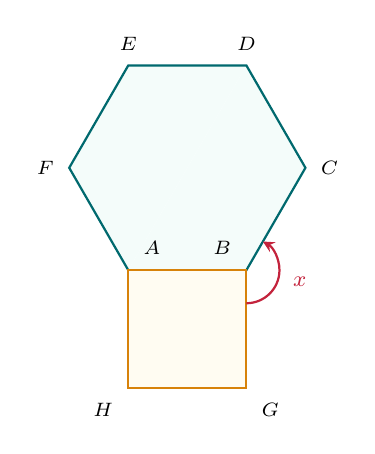
\begin{tikzpicture}[scale=1]
      % Regular Hexagon ABCDEF
      \coordinate (A) at (0, 0);
      \coordinate (B) at (1.5, 0);
      \coordinate (C) at (2.25, 1.3);
      \coordinate (D) at (1.5, 2.6);
      \coordinate (E) at (0, 2.6);
      \coordinate (F) at (-0.75, 1.3);
      
      \fill[brandTealBg] (A) -- (B) -- (C) -- (D) -- cycle;
      \fill[brandTealBg] (A) -- (D) -- (E) -- (F) -- cycle;
      \draw[thick, brandNavy] (A) -- (B) -- (C) -- (D) -- (E) -- (F) -- cycle;
      
      % Square ABGH drawn outside (below AB)
      \coordinate (G) at (1.5, -1.5);
      \coordinate (H) at (0, -1.5);
      \fill[brandGoldBg] (A) -- (B) -- (G) -- (H) -- cycle;
      \draw[thick, brandGold] (A) -- (B) -- (G) -- (H) -- cycle;
      
      % Nodes inside shapes to avoid collision with boundary lines
      \node[above right=2pt, font=\fontsize{7.5}{7.5}\selectfont] at (A) {$A$};
      \node[above left=2pt, font=\fontsize{7.5}{7.5}\selectfont] at (B) {$B$};
      \node[right=2pt, font=\fontsize{7.5}{7.5}\selectfont] at (C) {$C$};
      \node[above=2pt, font=\fontsize{7.5}{7.5}\selectfont] at (D) {$D$};
      \node[above=2pt, font=\fontsize{7.5}{7.5}\selectfont] at (E) {$E$};
      \node[left=2pt, font=\fontsize{7.5}{7.5}\selectfont] at (F) {$F$};
      \node[below right=2pt, font=\fontsize{7.5}{7.5}\selectfont] at (G) {$G$};
      \node[below left=2pt, font=\fontsize{7.5}{7.5}\selectfont] at (H) {$H$};
      
      % Angle arc around B from BG (-90 deg) to BC (60 deg)
      \draw[brandCrimson, thick, ->, >=stealth] ($(B)+(0, -0.42)$) arc (-90:60:0.42);
      \node[right=2pt, font=\fontsize{8}{8}\selectfont\bfseries, color=brandCrimson] at ($(B)+(0.4, -0.15)$) {$x$};
    \end{tikzpicture}
  \end{center}
\end{minipage}

\vspace{3pt}
% Problem 21
\noindent
\begin{minipage}{\linewidth}
  \exhead{21} មុំក្រៅនៃអដ្ឋកោណនិយ័តមួយមានរង្វាស់ $27^\circ$ តិចជាងរង្វាស់មុំក្រៅមួយនៃពហុកោណនិយ័តមួយដែលមាន $n$ ជ្រុង ។ ចូរគណនា $n$ ។
  \begin{center}
    \begin{tikzpicture}[scale=1]
      % Octagon vertex
      \begin{scope}[xshift=-1.4cm]
        \coordinate (O1) at (-1.0, 0);
        \coordinate (OV) at (0, 0);
        \coordinate (O2) at (45:1.0);
        \fill[brandTealBg] (O1) -- (OV) -- (O2) -- ($(O2)+(-0.7,0.3)$) -- cycle;
        \draw[thick, brandNavy] (O1) -- (OV) -- (O2);
        \draw[dashed, brandNavy!60] (OV) -- (0.9, 0);
        \draw[thick, brandCrimson, ->, >=stealth] ($(OV)+(0.36, 0)$) arc (0:45:0.36);
        \node[above right, font=\fontsize{6.5}{6.5}\selectfont\bfseries, color=brandCrimson] at ($(OV)+(20:0.38)$) {$45^\circ$};
        \node[below=1pt, font=\fontsize{7}{7}\selectfont\kml, color=brandNavy] at (0, -0.15) {អដ្ឋកោណ};
      \end{scope}
      
      % Polygon vertex (n=5)
      \begin{scope}[xshift=1.4cm]
        \coordinate (Q1) at (-1.0, 0);
        \coordinate (QV) at (0, 0);
        \coordinate (Q2) at (72:1.0);
        \fill[brandTealBg] (Q1) -- (QV) -- (Q2) -- ($(Q2)+(-0.6,0.3)$) -- cycle;
        \draw[thick, brandNavy] (Q1) -- (QV) -- (Q2);
        \draw[dashed, brandNavy!60] (QV) -- (0.9, 0);
        \draw[thick, koreaOrange, ->, >=stealth] ($(QV)+(0.36, 0)$) arc (0:72:0.36);
        \node[above right, font=\fontsize{6.5}{6.5}\selectfont\bfseries, color=koreaOrange] at ($(QV)+(36:0.38)$) {$72^\circ$};
        \node[below=1pt, font=\fontsize{7}{7}\selectfont\kml, color=brandNavy] at (0, -0.15) {$n = 5$ (បញ្ចកោណ)};
      \end{scope}
    \end{tikzpicture}
  \end{center}
\end{minipage}

\vspace{3pt}
% Problem 22
\noindent
\begin{minipage}{\linewidth}
  \exhead{22} មុំក្រៅនៃពហុកោណនិយ័តមួយដែលមាន $n$ ជ្រុង មានរង្វាស់ $30^\circ$ ច្រើនជាងរង្វាស់មុំក្រៅមួយទៀតនៃឆកោណនិយ័ត ។ ចូរគណនា $n$ ។
\end{minipage}

\vspace{4pt}
% Problem 23
\noindent
\begin{minipage}{\linewidth}
  \exhead{23} ពហុកោណនិយ័តមួយមានផលបូករង្វាស់មុំក្នុងស្មើនឹង $1440^\circ$ ៖\\
  \khlabel{ក} រកចំនួនជ្រុង $n$ នៃពហុកោណនិយ័តនោះ ។\\
  \khlabel{ខ} គណនារង្វាស់មុំក្នុងមួយ និងមុំក្រៅមួយនៃពហុកោណនោះ ។
\end{minipage}

\end{multicols}

\end{document}
